\documentclass[12pt]{article}
\usepackage[left=3cm, right=3cm, top=3cm]{geometry}
\usepackage[utf8]{inputenc}
\usepackage{amssymb}
\usepackage[dvipsnames]{xcolor}
\usepackage{amsmath}

\usepackage{natbib}
\usepackage{graphicx}
\usepackage{indentfirst}
\usepackage{array}
\usepackage{url}
\usepackage{hyperref}
\providecommand\phantomsection{}

\definecolor{ao}{rgb}{0.0, 0.42, 0.0}

\title{Review of deep learning models for cancer detection in computed tomography images}
\author{Candidate Number: 1016820 \\ Degree: Final Honour School of Mathematics and Statistics Part B}
\date{Hilary Term 2019}


\begin{document}

\maketitle


\centerline{\textbf{Abstract}}
Lung cancer is a leading cause of cancer deaths worldwide.  Computed tomography (CT) screenings can increase the detection rate of early-stage lung cancer and, as a consequence, decrease the mortality rate. Thus, in some countries, patients with an increased risk are advised to have annual low-dose CT examinations. Numerous computer-aided diagnosis (CAD) systems have been developed to assist radiologists with reading the CT scans and detecting any abnormalities. In this paper, we discuss the state-of-the-art systems that are based on deep learning methods. We focus in particular on the solutions submitted to the Data Science Bowl 2017 competition, which challenged the teams to develop an algorithm to predict the risk of lung cancer within one year from the CT screening. We also discuss commercial applications of these methods and their future challenges and opportunities.
\cleardoublepage
\tableofcontents
\cleardoublepage
\section{Introduction}
\subsection{Lung cancer}
Lung cancer is the third most common type of cancer worldwide, and it is the most common cause of death from cancer \citep{CancerUK}. According to the Cancer Research UK, the estimated lifetime risk of lung cancer is 7\% for women and 8\% for men born after 1960 in the UK. It is predicted still to be a leading cause of death from cancer in 2035  \citep{smittenaar2016cancer}. It is of high importance to diagnose lung cancer early, as it significantly increases the chance of surviving. The overall five-year survival rate is only 9.5\%, but, if lung cancer is diagnosed at stage I, the five-year survival rate rises to 35\% \citep{CancerUK}. 

Lung nodule detection is an essential part of lung cancer diagnosis \citep{armato2011lung}. A lung nodule refers to a small mass of tissue in the lung. Nodules can be detected on chest radiography scans or computed tomography scans, where they appear as round, white shadows. Nodules can be either benign, in which case they are an abnormal tissue that serves no purpose and is noncancerous, or they can be malignant. Thus, nodule classification is another key step of lung cancer diagnosis.

Screening for lung cancer with low-dose CT increases the detection rate of lung cancer at an earlier stage when it can be more effectively treated \citep{caroline2014lung}. It has also been shown to obtain better results than radiography (i.e., it demonstrated a reduction in death from lung cancer). However, there are several drawbacks to low-dose CT screening that include costs of wide-spread testing and the radiation risks. Therefore, screening centres should carefully determine the population to be screened (e.g., according to the recent guidelines, only people with increased risk of lung cancer should be considered for this examination). Other drawbacks of this method include an additional burden falling onto oncologists and a chance of incidental false positive findings. To address these issues and to provide support for doctors, CAD systems have been developed over the last few decades.

\subsection{Computer-aided diagnosis systems}
Computer-aided diagnosis (CAD or CADx) systems are computer programs aimed at assisting doctors in the interpretation of medical images. In the case of lung nodule detection, CAD systems could support doctors by providing a second opinion or, possibly, even take the burden entirely off radiologists. As discussed in the next section, doctors are not entirely accurate in lung nodule detection on CT images so that CAD systems could become more accurate than humans.

Deep learning methods have been the foundations of the most promising CAD systems. They are far superior to traditional machine learning methods, as they can identify and learn complex features from raw data. As Bakator and Radosav presented in \citep{bakator2018deep}, typical applications of deep learning in medicine include diagnosis, segmentation, detection and classification, while the most frequent data sources are CT and MRI data. They have found convolutional neural networks (CNNs) to dominate among deep learning methods. CNNs are a specialised kind of neural networks that process well image data. Due to their significance in lung cancer detection, they will be described in detail in Section 2.2.1, whilst numerous CNN-based models will be discussed later. According to Ahmad et al., it is only a matter of time before machine learning will be ubiquitous in healthcare \citep{ahmad2018interpretable}.

\subsection{Lung Image Database Consortium (LIDC) data}
 In order to allow for the comparison of different CAD systems and to encourage their development, in 2007, the Lung Image Database Consortium (LIDC) was introduced by the National Cancer Institute in the United States \citep{mcnitt2007lung}. LIDC is a publicly available database of thoracic CT scans that were marked for the location and spatial extent of lung nodules. We can see sample images from the database in Figure 1 and close-ups of an image containing a malignant nodule in Figure 2. Each scan was reviewed by four radiologists
\begin{figure}[h!]
\centering
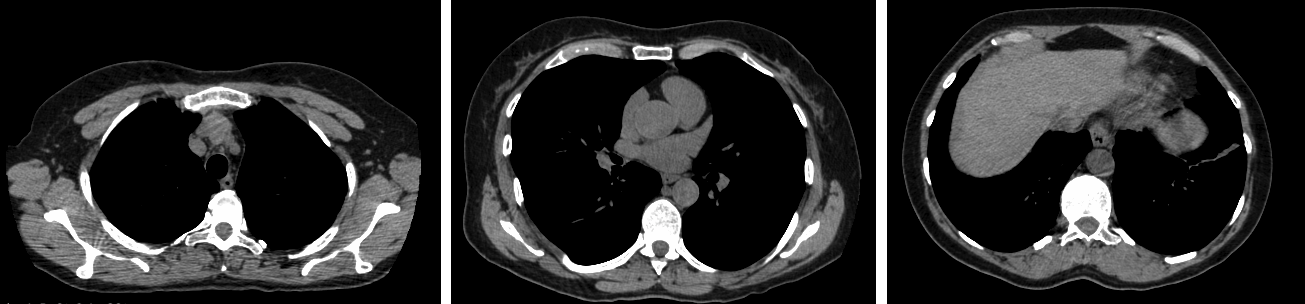
\includegraphics[scale = 0.335]{lung.png}
\caption{Sample pictures in the z-axis (left: the top part of the chest; centre: the middle part; right: the bottom part) coming from the same CT scan from the LIDC dataset.}
\end{figure}
\begin{figure}[h!]
\centering
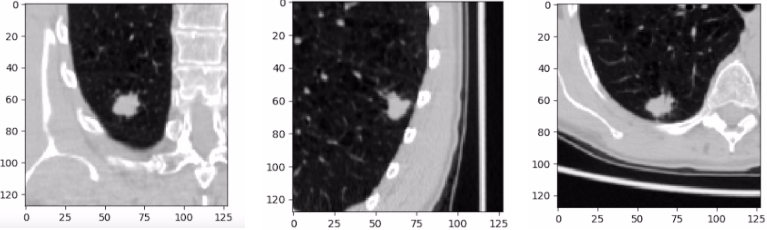
\includegraphics[scale = 0.575]{nodule.png}
\caption{A close-up of a malignant nodule, each picture presents a view in a different axis (left: x-axis; centre: y-axis; right: z-axis), figure from \citep{deepbreath}.}
\end{figure}
 using the following process: in the first (``blinded") stage, each radiologist reviewed the scans independently. Then the results from all reviews were presented to each radiologist, and in the second (``unblinded") stage, they were able to compare their annotations with the reviews of the other three radiologists and give their final review that was then saved in the database.

Initially, it contained data from approximately 100 patients, and it was continuously expanded until 2011 \citep{armato2011lung}. According to this paper, LIDC contains 1018 cases, each one including images from a clinical thoracic CT scan and an associated XML file with the result of the image annotations process described above. Marked lesions belong to one of three categories, which are defined in the following way: 
\begin{itemize}
    \item nodule $\geq 3 $ mm: a lesion considered to be a nodule with the diameter in the range 3–30 mm (it is stated that 30 mm is an acceptable upper limit for a nodule size),
    \item  nodule $< 3$ mm: a lesion considered to be a nodule with the diameter less than \\3 mm that is not clearly benign,
    \item non-nodule $\geq 3$ mm: any other pulmonary lesion; with the diameter greater than or equal to 3 mm that does not reveal features attributed to a nodule.
\end{itemize}


\begin {table}
\caption {Summary of number of nodules identified by LIDC radiologists across all 1018 scans. Based on the table from \citep{armato2011lung}. } \label{tab:title} 
\begin{center}
\begin{tabular}{ | m{8cm} |  m{3.5cm} | } 
\hline
\textbf{Nodule $\pmb{\geq }$ 3 mm  or nodule $\pmb{ <}$ 3 mm:} & \\
\hline
Marked by at least one radiologist & 7371 nodules \\
Marked by all four radiologists & 2562 nodules\\
Marked by all four radiologists with the same label (nodule $\geq 3 $ mm  or nodule $ <$ 3 mm) & 1940 nodules\\
\hline
\textbf{Nodule $\pmb{\geq }$ 3 mm:} &\\
\hline
Marked by at least one radiologist & 2669 nodules\\
Marked by all four radiologists & 928 nodules\\
\hline

\end{tabular}
\end{center}
\end{table}

Table 1 presents a summary of radiologists' annotations. We can notice that there were significant differences in their opinions. There are 7371 points marked by at least one radiologist as a nodule (either $\geq 3$ mm or $< 3$ mm), and only 2562 points (34.8$\%$) were marked as a nodule (of either size) by all four radiologists. Therefore, there was a disagreement between the readers in 65.2$\%$ of all marked points, even though they could see markings from the other three readers, and they were allowed to make corrections. Moreover, only 1940 nodules  (26.3 $\%$ of all marked points) were assessed the same mark (either nodule $\geq 3 $ mm or nodule$< 3$ mm) by all four radiologists.   

All annotations are saved in XML files (there is one file for each patient), but it is stated that the order in which the radiologist's mark appears is not consistent across XML files. Therefore, it is not possible to draw any conclusions about reader consistency based on the whole dataset. However, Opfer and Wiemker presented a very detailed and thorough validation study of the initial dataset in \citep{opfer2007performance}, which contained only 93 cases at that time. They found the sensitivity of each reader to be between 0.55 and 0.79, and the number of false positives per scan to be between 0.76 and 2.15 for each radiologist. These values depend on the radiologist and on what is assumed to be a ground truth. 


\section{Methods}

\subsection{Machine learning}
Machine learning is one of today's fastest growing technical fields \citep{Jordan255}. Its applications can be found in face recognition, natural language processing, fraud detection, autonomous cars and many more.

Kevin Murphy defined machine learning in the following way: `` The goal of machine learning is to develop methods that can automatically detect patterns in data, and then to use the uncovered patterns to predict future data or other outcomes of interest." \citep{murphy2012machine}. Another fundamental aspect of machine learning, as Jordan and Mitchell noted in \citep{Jordan255}, is the ability to improve through experience. 

A learning problem can be defined as the problem of improving some measure of performance when executing some task through some type of training experience \citep{Jordan255}. For example, in learning to classify nodules as benign or malignant, the task is to assign a label of ``benign" or ``malignant" to every nodule given (e.g., on the CT scan). The performance metric might be the accuracy of this malignancy classifier, and the training experience might consist of a collection of CT scans with marked nodules, each labelled in retrospect as malignant or not. Alternatively, one can use a different performance metric or assign a higher penalty for classifying a malignant nodule as benign than when a benign nodule is classified as malignant. This can be done by designing a desirable loss function.

Assume that we train a model that aims to predict an outcome $y$ using observed features $\vec{x}$. Suppose that for some value $\vec{x}_1$, this algorithm made a prediction $\hat{y_1}=f(\vec{x}_1)$. To measure how good this prediction is, we can introduce a loss function $L: Y \times Y \rightarrow R$ that compares the output $\hat{y_1}$ with the true value of $y_1$. For regression problems, typical examples are squared loss and absolute loss. For classification problems that output a vector of probabilities $\hat{p}(k)$ for $\vec{x}$ belonging to the class k, it is common to use a log-likelihood loss (also called Log-Loss) $L(Y, \hat{p})= -\log(\hat{p}(Y))$. 

For classification algorithms that output only the predicted class, there are other performance measures available. To define them, we will use the confusion matrix presented in Table 2. Let TP, FP, TN and FN denote the number of examples marked as true positives, false positives, true negatives and false positives, respectively. Then, we can define the following measures of performance:

\begin {table}
\caption {Confusion matrix. The top row presents the true state of the value y, and the left column presents the prediction made by an algorithm. } \label{tab:title} 
\begin{center}
\begin{tabular}{|c|c|c|}
  \hline
  \text{prediction $\smallsetminus$ true state} & 1 & 0 \\ 
  \hline
  1 & \text{True positive} & \text{False positive} \\ 
  \hline
  0 & \text{False negative} & \text{True negative}\\
  \hline
 \end{tabular}
 \end{center}
 \end{table}


\begin{itemize}
    \item Accuracy = (TP + TN) / (TP + FP + TN + FN)
    \item Sensitivity (also called Recall) = TP / (TP + FN)
    \item Precision = TP / (TP + FP)
    \item F1 score (also called Dice's coefficient) = 2TP/(2TP+FP+FN), the harmonic mean of precision and recall
\end{itemize}
Other performance measures are the following:  specificity and false positive rate. Accuracy is often used, but in some cases, other measures carry more information about the performance of the model. A measure equivalent to accuracy is the error rate (proportion of examples for which the model produces an incorrect output); it is often referred to as the expected 0-1 loss. Another common measure is the area under the receiver operating characteristic curve (AUC). It can be interpreted as the probability that the model ranks a random positive example more highly than a random negative example. The receiver operating characteristic curve plots the sensitivity against the specificity of a binary classifier as the threshold for discrimination is varied. 

However, the performance of an algorithm measured on the training set is not a good indicator of predictive performance on unseen data due to the problem of over-fitting. Thus, a conventional technique is to divide the training dataset into two parts: training and validation. Then, after training a range of models on the training set, one can validate their performance on the independent validation set, and select the one having the best predictive performance. 

In many applications, however, the supply of training data is limited, and we would like to use as much of the available data as possible for training in order to build an accurate model. On the other hand, if the validation set is small, it will give a weak predictive performance due to the significant amount of noise. A solution to this trade-off is k-fold cross-validation \citep{bishop2006pattern}. We divide the training set into the k parts; and then the learning process consists of k iterations, every time we use different (k-1) parts for training and the last part for validation. Following that, we average the predictive performance to obtain a final score.  If we take k to be to the total number of data points, we will obtain a technique called leave-one-out. 


\subsection{Deep learning} 
The following section is written based on \citep{goodfellow2016deep}. For many tasks, it is difficult to know which features should be extracted (nodule detection is a good example). One solution to this problem is to use machine learning to discover not only the mapping from representation to output but also the representation itself. This approach is known as representation learning. However, it can be complicated to extract high-level, abstract features from raw pixel data. Deep learning solves this central problem in representation learning by introducing representations that are expressed in terms of other, simpler representations. Thus, deep learning models consist of many layers (hence the name deep learning), where the initial layers usually detect simple features (e.g., edges in the pictures), and the following layers detect more and more complex features. 

The goal of a neural network is to approximate some function $f^{*}: X \rightarrow Y$, given a training set of data points $(\vec{x}, y)$ where $f^*(\vec{x})=y$. The neural network defines new mappings $f: X \rightarrow Y$, and chooses the one the most similar to the original $f^*$. In a standard neural network, the information flows from data $\vec{x}$ through the intermediate computations used to define $f$, to the output $y$. This type of network is called a feedforward network. Alternatively, one could implement feedback connections in the network, which would feed the output of the model back to itself. These networks are called recurrent neural networks.

Neural networks are called networks, because they are usually represented as a composition of different functions, which can be graphically represented in the form of a directed acyclic graph describing the way in which the functions are composed. For example, we might have $f(\vec{x})=f^{(3)}(f^{(2)}(f^{(1)}(\vec{x})))$. In this case, $f^{(1)}$ is called the first layer of the network, $f^{(2)}$ is called the second layer, and so on. The first layer is often called the input layer, and the final one is called the output layer. The layers in-between are called hidden layers, because training data do not specify their desired output. The depth of the network is defined as the number of functions composed. 


Neural networks are called neural, because they are inspired by the functioning of the brain. Each hidden layer is usually vector-valued, while each element of the vector can be considered a neuron.  It receives information from many other neurons in the previous layer, and it computes its own activation value.  A sample network with one neuron is presented in Figure 3. 

\begin{figure}[h!]
\centering
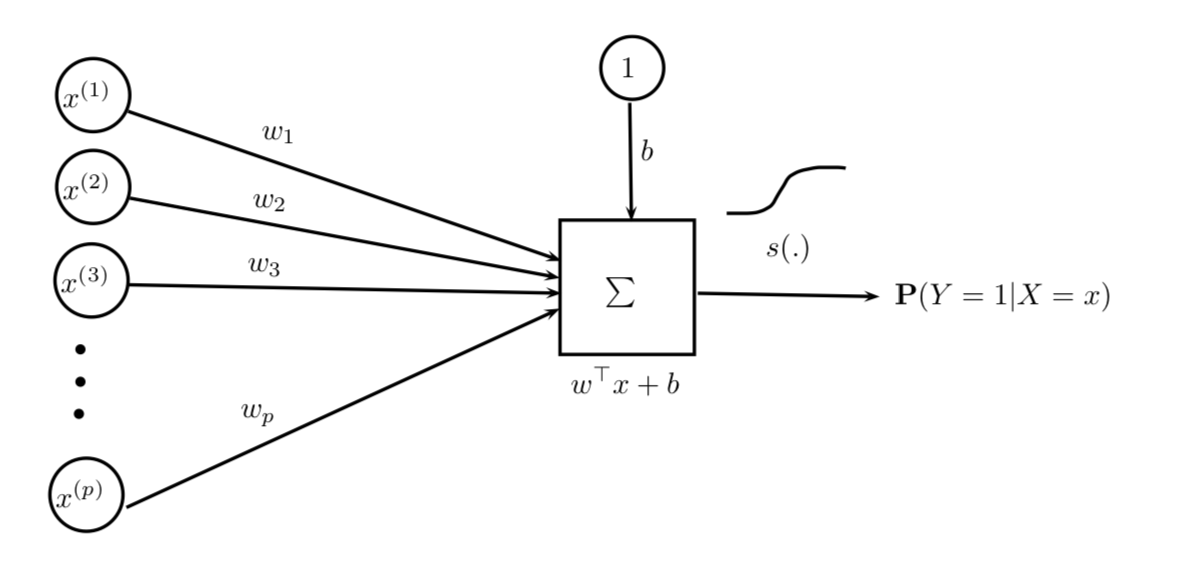
\includegraphics[scale = 0.3]{NN.png}
\caption{A neural network with one neuron and input $x_1,\ldots, x_p$. Values $w_1,\ldots, w_p$ are model weights, $b$ is the bias term, $w^Tx + b$ is the activation value and $s(.)$ is called activation (or tansfer) function; it returns the output. This figure comes from \citep{lectures}. }
\end{figure}

An activation function is assigned to each neuron. It is used to transform the input data into a desired output. The default recommendation is to use the rectified linear unit (ReLU), defined as $f(x) = max \{0,x\}$. Other typical activation functions are the sigmoid function, defined as $\sigma(x) = 1 / (1 + e^{-x})$, hyperbolic tangent, defined as $\tanh(x) = (1-e^{-2x}) / (1 + e^{-2x})$. 
Two simple examples of output layer for a multi-class classification are maxout, defined as $f(\vec{x}) = \max_i x_i$, returning the single most likely class, and softmax, given by $f_i(\vec{x}) = e^{x_i}/(\sum_{j=1}^J e^{x_j})$, returning for each class the probability that the input belongs to this particular class. The way the softmax is defined guarantees that the returned probabilities always add up to 1. 

The number of layers and neurons are determined by the author based on their experience and intuition. All other parameters are learned by the neural network: it aims to find such a set of parameters that minimises the total loss. As in the case of traditional machine learning, it can be done through a back-propagation, using a gradient descent algorithm or one of its variations.

\subsubsection{Convolutional neural networks}
Convolutional neural networks (CNNs) are a type of neural networks specialised in processing data with a grid-like topology, in particular, image data. They are inspired by the organisation of cats' visual cortex \citep{miotto2017deep}.

Convolution is a mathematical operation defined as $(x \star w)(t)= \int x(a)w(t-a)da $, where $x(t)$ usually represents the input, and $w(t)$ is an appropriately chosen kernel. In CNNs, there is at least one layer in which standard matrix multiplication is replaced by convolution. It leverages three important ideas: sparse interactions, parameter sharing and equivariant representations. 

A typical convolutional layer consists of three stages: convolution stage,  detector stage and pooling stage, such as max pooling operation, which returns the maximum output within a rectangular neighbourhood. The last step helps to make the representation invariant to small translations of input, and it can reduce the computational cost by downsampling the number of neurons. To prevent the data from shrinking, a padding layer can be introduced, which adds zeros at the boundaries of an input. The last common building block of CNNs is a fully connected layer, which connects all input neurons with all output neurons. 


\section{Data Science Bowl 2017}
\subsection{Problem description}
In 2017, a lung cancer prediction challenge called Data Science Bowl (DSB) was announced on the Kaggle website \citep{kaggle}. The following problem description can be found on the competition website:
\\\\ 
\textit{In this dataset, you are given over a thousand low-dose CT images from high-risk patients in DICOM format. Each image contains a series with multiple axial slices of the chest cavity. Each image has a variable number of 2D slices, which can vary based on the machine taking the scan and patient. The DICOM files have a header that contains the necessary information about the patient id, as well as scan parameters such as the slice thickness. The competition task is to create an automated method capable of determining whether or not the patient will be diagnosed with lung cancer within one year of the date the scan was taken. The ground truth labels were confirmed by pathology diagnosis.}\\

An intuitive approach to this problem is to detect all lung nodules first and then to calculate malignancy probability for each nodule. Subsequently, based on this information one can try to predict the probability of the patient being diagnosed with lung cancer within one year.


The training data contained 1600 high-resolution chest CT scans with slice thickness less than 3mm. Most participants used external training data, coming from the LUng Nodule Analysis (LUNA) Grand Challenge 2016 \citep{luna}, which contained approximately 900 additional scans and essential information about the locations of each nodule in the CT scan. The LUNA competition aimed to detect lung nodules automatically in CT images. LUNA dataset is a subset of the LIDC dataset, but it does not contain the annotations made by the radiologists (other than locations of nodules and some non-nodules). Some contestants used LIDC data as well.

The first step of a solution to an image analysis problem is data preprocessing. It usually includes data cleaning, instance selection, normalisation, transformation, feature extraction and selection. Data normalisation was particularly substantial, because different CT machines have varying slice thickness, and they may produce pictures of variable resolution. In most cases, the data were scaled so that one voxel (volumetric pixel) represented 1mm$^3$. Data transformation usually included normalising values of each voxel (initially given in Hounsfield Units \--- a standard quantitative scale for describing radiodensity). Moreover, lung segmentation was a vital preprocessing step, because each CT scan represents approximately a 300 mm x 300 mm x 400 mm section of a person's chest, while a lung nodule is around 10 mm in diameter (Average nodule diameter is 13.68mm in the DSB dataset and 8.31mm in the LUNA dataset \citep{liao2017evaluate}). Therefore removing non-lung tissues from the images can significantly improve the performance of the algorithm, and it can also decrease its running time. Sample segmentation tutorials were posted on the competition website to help participants to get started.

A common difficulty for a 3D object detection task is a GPU memory constraint. For object detection in 2D images, it is possible to use an entire image as an input to the models during training. However, it is not possible to use whole lung scans (even after segmentation) as an input for 3D nodule detection models, because even a single sample would exceed the limit of a standard GPU memory  \citep{liao2017evaluate}. Thus, scans have to be divided into small cubic parts called patches, and a model can be trained to detect nodules in these patches.

\subsection{Discussed submissions}
In this section we are going to focus on discussing the following solutions:
\begin{enumerate}
\item ``grt123" solution by Liao et al., described in the paper \citep{liao2017evaluate}. They won the competition with a Log-Loss of 0.39975,
\item Solution by Julian de Wit and Daniel Hammack, described in the blog posts \citep{dewit},\citep{hammack} and Hammack's technical report \citep{Hammack2}. They achieved second place with a Log-Loss of 0.40117,
\item ``Deep Breath" solution by Verleysen et al. described in the blog post \citep{deepbreath} written by E. Vansteenkiste. They achieved $9^{th}$ place and a Log-Loss of 0.43872.
\end{enumerate}
The code for the top ten solutions for the competition is available on the website \citep{top10}. The Log-Loss function used to score the solutions can be expressed by the following formula: 
$$\textrm{LogLoss} = - \frac{1}{n} \sum_{i=1}^n \left[ y_i \log(\hat{y}_i) + (1 - y_i) \log(1 - \hat{y}_i)\right],$$
where n is the number of patients in the test set; $\hat{y}_i$ is the predicted probability of the image belonging to a patient with cancer; $y_i$ is 1 if the diagnosis is cancer, 0 otherwise and log() is the natural logarithm.

\subsection{Verleysen et al.'s solution}
In the first step, Verleysen et al. assigned to each voxel the probability that it belongs to a nodule, using a nodule segmentation network based on a U-net architecture (which was first introduced in \citep{ronneberger2015u}). They used 64 x 64 x 64 patches (height x length x width, in pixels, the same notation is used in what follows) as an input. As an optimisation objective, the F1 score (described in Section 2.1) was chosen.

To increase the amount of training data, the team used the additional images from the LUNA dataset and they applied a method called data augmentation. That is, the authors applied image transformations to the scans, and added the copies to the training set as new samples. There are 48 lossless transformations (rotations and flips) of a 3D object, and they are equivalent to the isometries of a cube. Sometimes, if more data is needed still, translations or lossy transformations are used as well. Even though a human might be able to tell that there are many copies of each scan in the dataset, a neural network does not recognise this, and it treats each copy as a new example. If a model returns different answers for different copies of the same scan, the average of the results can be used as the final outcome. The benefits of data augmentation in image classification have been presented in detail in \citep{wong2016understanding}; they include improved performance and reduced overfitting.

In the next step, the team focused on using the output from the previous model to detect the centres of the nodules. To find the nodules, they were looking for groups of voxels with high nodule probability. This way, they obtained a list of nodule candidates, and they proceeded to the false positive reduction. To achieve this goal, they decided to add a lung segmentation step before the detection and to train an expert network for this purpose.

Verleysen et al. initially built a lung segmentation network similar to the one proposed in the tutorial available on the competition website \citep{kaggle}. However, they noticed some problems with this method, some of which were caused by the limitations of a 2D segmentation algorithm. In particular, nodules attached to the outer wall of the lungs were unintentionally removed during this segmentation process. Therefore, the team decided to build a different 3D segmentation model, which cut out the non-lung part from the convex hull built around the lungs. They found the new algorithm to perform better in the edge cases that caused problems with the previous method.

To further reduce the number of false positives, an expert network was trained to predict if a given nodule candidate is indeed a nodule. They used data (a list of false and true positives for each patient) from the false positive reduction track of the LUNA challenge. The architecture of this network was based on a ResNet network (which was first introduced in \citep{he2016deep}); the authors used patches of size 48 x 48 x 48 and applied data augmentation. 

Once they discovered the radiologists' annotations included in the LIDC dataset, they built the next model to predict the malignancy of individual nodules. Subsequently, they tried many data aggregation strategies to produce the final cancer prediction; below we present two methods that they found to be the most successful:
\begin{enumerate}
\item P(developing cancer in a year) = 1 - $\prod$ P(nodule is benign), where the product is taken over all nodules detected for the particular patient. This approach assumes that if all found nodules are clearly benign, then the cancer probability is 0. On the other hand, if at least one nodule is classified as malignant, then the cancer probability will be 1. This idea is similar to the noisy-or network described in Section 3.5.
\item Log Mean Exponent. When this aggregation method is applied, the most malignant nodules contribute the most to the cancer probability.
\end{enumerate}

\subsection{De Wit and Hammack's solution}
Julian de Wit and Daniel Hammack were working independently at first, and decided to combine their solutions towards the end of the competition period. Their models were combined by taking a weighted average of cancer predictions returned by each of them.

\subsubsection{Hammack's solution}
The first step of Hammack's method, after data preprocessing and lung segmentation, is a detector of nodule candidates \--- a high-sensitivity model detecting patches containing nodules. Due to the high-sensitivity, it returned many false positives, but it should not have missed any nodules. Input patches were of size 64 x 64 x 64. Regions not detected by the model were classified as ``normal tissue" and removed. Each scan was limited to have between 1 and 50 ``abnormal regions''. Overall, the preprocessing and the detector reduced the volume to be searched by eight times.   

Hammack also used additional iamges the LUNA dataset for training, and he found radiologists' annotations from the LIDC dataset to be particularly useful. He chose to use the following nodule attributes in the model:  malignancy, diameter, spiculation, lobulation. He trained a few different models predicting these attributes and then created a list of 18 features (derived from these attributes and image data), which were fed into diagnosis classifier consisting of L1-penalised logistic regression and extremely random trees regressor fit. One of the included features was the location of the nodule in the z dimension, as Hammack has noticed that nodules found in the upper lobe were more likely to be malignant. This observation has been earlier discussed in \citep{perandini2016distribution}, where statistical significance of nodule location was evaluated with the Chi-square test.

He used lossless and lossy data augmentation. He also applied a method called curriculum learning. It aims to mimic a way in which humans learn: starting with simple, easy examples, we gradually improve our skill and continue learning with more and more complex tasks. In terms of machine learning, it usually means to first train a model on examples that are easy to classify and then to train the same model on the rest of the training set. Hammack first trained a model on smaller patches of size 32 x 32 x 32, because they were faster to train, as they are eight times smaller, and then the same model was trained on the 64 x 64 x 64 patches.

Finally, Hammack decided to build many models that differ in aspects such as the loss function, the activation function, fraction of data was used for training and combined results returned by all of them. This method is called model ensembling. The results can be aggregated by, for example, a weighted average of all responses or by majority voting. If there is enough variety between the models, their ensemble is expected to perform better than any of the models on its own.

\subsubsection{De Wit's solution}
De Wit's approach is similar to Hammack's, he also used the LUNA dataset and the annotations from the LIDC dataset. We can see a high-level overview of this method in Figure 4. However, as opposed to Hammack, he used a 1-stage multi-task learning approach. De Wit's used the same network to detected nodules in the 32 x 32 x 32 patches and to predict their malignancy. The architecture was based on C3D network (which was first introduced in \citep{jia2014caffe}).
\begin{figure}[h!]
\centering
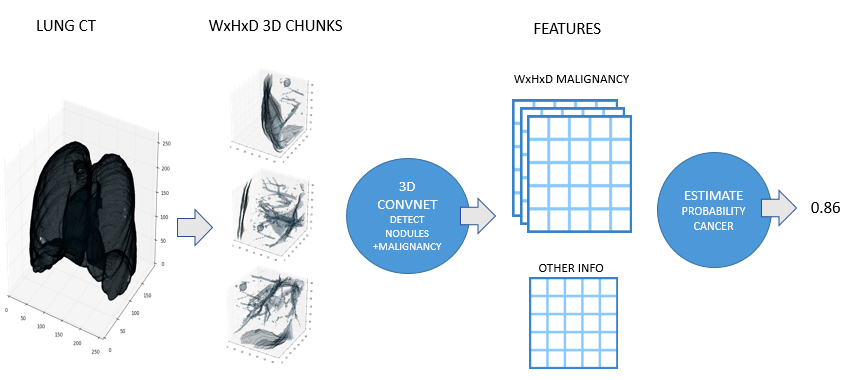
\includegraphics[scale = 0.45]{julian.png}
\caption{A high-level overview of de Wit's model, figure from \citep{dewit}. }
\end{figure}


The author noticed the same segmentation problem as Verleysen et al. \--- nodules attached to the outer walls of the lung and were unintentionally removed. Therefore, he decided to skip the segmentation step completely. To train the network to ignore everything outside the lungs, he created a list of 150000 negative candidates from the non-lung tissue.

De Wit also tried detecting emphysema. Although it did not improve the performance of the model, we find it worth mentioning. Emphysema is a destruction of the lung, caused mainly by smoking cigarettes, which is associated with a higher risk of cancer, and it is visible on the CT scans.   


\subsection{Liao et al.'s solution}
The first part of Liao et al.'s solution is a novel volumetric one-stage end-to-end convolutional neural network for 3D object detection, which detects potentially malignant nodules. The second part is a neural network with the integrated leaky noisy-or gate for cancer prediction. Both components are a modified version of a U-net, and they share the same backbone. 

In the first part (suspicious nodule detection), 128 x 128 x 128 patches were used as an input. The training set was constructed in the following way: 70\% of the patches must contain a nodule, the other 30\% were cropped randomly from the lung scans. An overview of the network layout is presented in Figure 5.

\begin{figure}[h!]
\centering
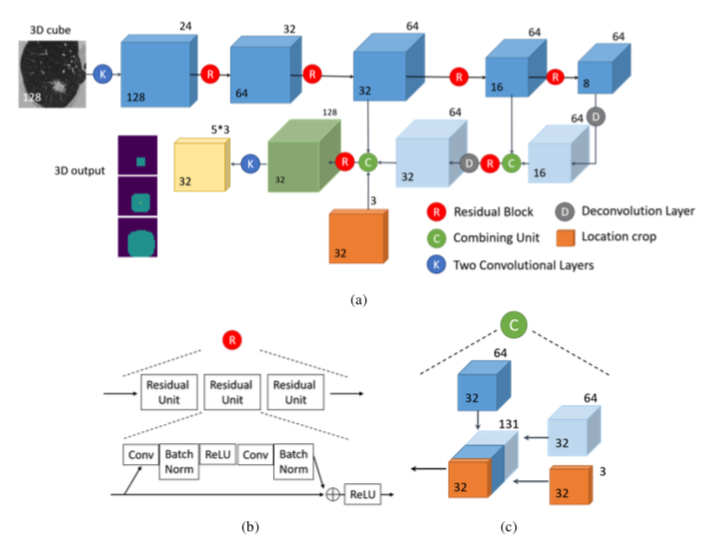
\includegraphics[scale = 0.57]{liao.png}
\caption{Figure from \citep{liao2017evaluate}, original description: ``The nodule detection net. (a) The overall network structure. Each cube in the figure stands for a 4D tensor. Only two dimensions are indicated in the figure. The number inside the cube stands for the spatial size (Height = Width = Length). The number outside the cube stands for the number of channels. (b) The structure of a residual block. (c) The structure of the left combining unit in (a). The structure of the right combining unit is similar but without the location crop." }
\end{figure}

The team used data augmentation to prevent overfitting, but they only used left-right flips and rescaling (ratio between 0.8 and 1.15). They found that other transformations (axes swapping and rotation) did not cause significant improvement. 

Liao et al. used a region proposal network as an output layer of a fast R-CNN network, enabling them to generate nodule proposals (with assigned confidence levels) directly. Region proposal networks (RPNs) were first introduced in \citep{ren2015faster}. They reduce region proposal computation (the bottleneck of the state-of-the-art object detection networks of that time). RPNs share full-image convolutional features with the detection network, thus enabling nearly cost-free region proposals. They simultaneously predict object bounds and probability scores at each position. 


The authors used hard negative mining to reduce false positives. After training the algorithm, they picked some of the falsely detected examples and added them to the training set as negative examples. Then, they retrained the classifier and noticed an improvement in the performance.



Contrary to Verleysen et al. and de Wit and Hammack, Liao et al. decided to reuse the neural network from the nodule detection part for the evaluation of the overall cancer probability. For each patient, five nodule candidates with the highest confidence levels were selected and used for cancer prediction. Four different methods of aggregating the data were explored to obtain a single prediction score: feature combining, MaxP, Noisy-or, Leaky Noisy-or. The last method yielded the best results (smallest loss). An overview of the nodule classifier network and the four different aggregation methods is presented in Figure 6.

\begin{figure}[h!]
\centering
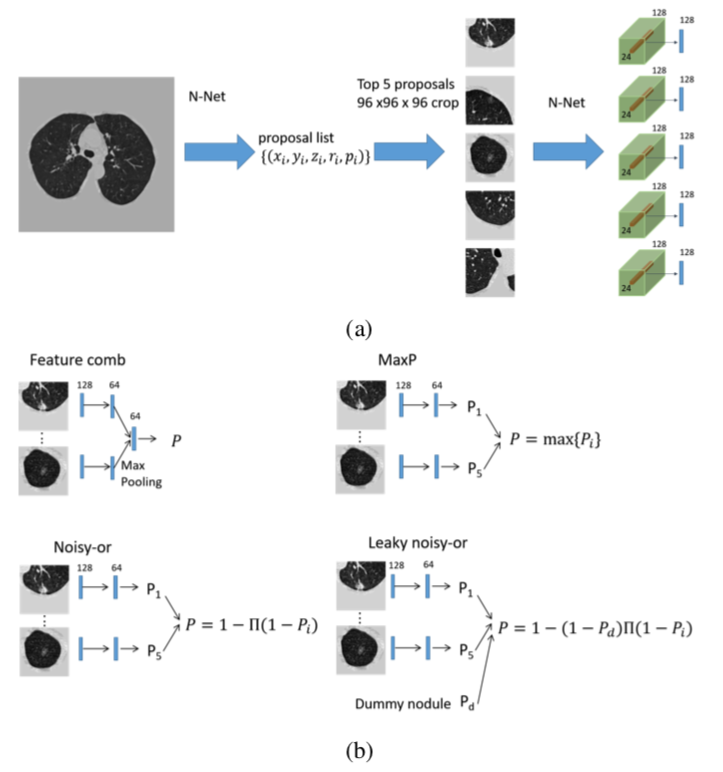
\includegraphics[scale = 0.45]{liao2.png}
\caption{Figure from \citep{liao2017evaluate}, original description:  ``Illustration of the case classifier. (a) The procedures of getting proposals and features of proposals. (b) Different multi-nodule information integration methods." }
\end{figure}

Noisy-or networks are often explained using a very accurate example of diseases and symptoms \citep{arora2017provable}. We present below the idea behind them.

Assume there are m possible diseases and n possible symptoms. Consider a particular patient and define hidden binary variables $d=(d_1, d_2, \ldots, d_m)$, where for each $i=1, 2, \ldots m$, we have $d_i = 1$ if the patient has disease i and, 0 otherwise; binary variables $s=(s_1, s_2,\ldots, s_n)$ where for each $i=1, 2, \ldots ,n$ we have $s_i = 1$ if the patient has symptom i, and 0 otherwise. Variables corresponding to the diseases are considered as hidden because a doctor can only observe symptoms, not the diseases themselves. Assume that,
\begin{itemize}
\item  hidden variables $d_1, d_2, \ldots, d_m$ are independent and have Bernoulli distributions,
\item  conditioned on d, variables $s_1, s_2,.., s_n$ are independent and have exponential distributions with known weights $W_{j,i}$, where (W is a non-negative $n \times m$ matrix): for a single symptom we have that $P(s_i=1|d_j)= 1 - \exp(W_{j,i}d_j)$ is the probability that disease j activates symptom i.
\item symptom $s_i$ is activated if at least one of the diseases activated it (which explains the name of the network: noisy-or).
\end{itemize}
An immediate calculation gives: $$P(s_i=1|d) = 1- {\displaystyle \prod_{j=1}^{m} \exp(-W_{j,i}d_j)}.$$ 
\\The conditional distribution $P(s|d)$ is given by:
$$P(s|d) = {\displaystyle \prod_{i=1}^{n} \{(1 - \prod_{j=1}^{m} \exp(-W_{j,i}d_j))^{s_i}(\prod_{j=1}^{m} \exp(-W_{j,i}d_j))^{1-s_i}\}}.$$
\\The goal of this model is to find the probability of a patient having a particular disease given the observed symptoms. 
\\\\In the lung cancer prediction case, we want to predict the probability of a patient having lung cancer (within a year from the scan) given the observed nodules and their corresponding cancer risks. In \citep{liao2017evaluate}, the following equation was used for calculating the final cancer probability:
\\$P = 1 - {\displaystyle \prod_{i=1}^{5} (1-P_i)}$, where $P_i$ is the cancer probability of the i-th nodule.

The model described above has a particular weakness when applied to this case. Sometimes the lung cancer can appear even if none of the nodules has been found be malignant (either because the malignant nodules were missed or because they were not there yet at the time of the CT examination). Then, the model would assume that the benign nodules that were found were the cause of cancer, and this is unwanted behaviour. The leaky noisy-or network is a modification of the previous model that addresses this problem. A new artificial nodule was introduced with $P_d$ as its cancer probability. This value is learned automatically during the learning process.  The new equation for the final cancer probability is: \\$P = 1 - (1-P_d){\displaystyle \prod_{i=1}^{5} (1-P_i)}.$


\subsection{Comparison of results}
In Sections 3.3-3.5 we presented three successful approaches to the same problem; they were all based on the state-of-the-art methods. De Wit, Hammack and Verleysen et al. admitted that due to the time constraint imposed by the competition, they did not manage to fine-tune every part of their models, and there is still room for improvement; Liao et al. introduced small modifications to their model after the competition. 
Table 3 presents a detailed comparison of the three solutions. 

\begin {table}
\caption {Comparison of the three DSB submissions discussed in this section.} \label{tab:title} 
\begin{center}
\begin{footnotesize} 
\begin{tabular}{ | m{2.2cm} |  m{3.9cm} |  m{3.9cm} |  m{3.9cm} | } 
\hline
& \textbf{Verleysen et al.} & \textbf{De Wit and Hammack} & \textbf{Liao et al.}  \\ 
\hline
\textbf{Competition result} & 9$^{th}$ place & 2$^{nd}$ place & 1$^{st}$ place\\
\hline
\textbf{External training data} & LUNA and LIDC & LUNA and LIDC & LUNA  \\ 
\hline
\textbf{Lung segmentation method} & 3D segmentation (preserved nodules attached to the lung wall) & De Wit: no lung segmentation, Hammack: standard 2D segmentation &   segmentation mask combined with its convex hull (preserved nodules attached to the lung wall) \\
\hline
\textbf{Nodule detection method} & Assign nodule probability to each voxel, produce nodule candidates, reduce FP rate  &De Wit: 1-stage model for nodule detection and malignancy estimation, Hammack: 2-stage model for nodule detection and prediction of mutltiple features &  3D region proposal network \\ 
\hline
\textbf{Cancer prediction method} & linear model based on nodule malignancy &De Wit: tree model, Hammack: linear model based on 18 handcrafted features & Leaky Noisy-or network \\
\hline
\textbf{Architecture} & Modified U-net for nodule segmentation, ResNet-like for FP reduction & De Wit: modified C3D, Hammack: ResNet-like & Modified U-net\\
\hline
\textbf{Size of the input patches} & 64 x 64 x 64 & De Wit: 32 x 32 x 32, Hammack: 64 x 64 x 64 & 128 x 128 x 128 \\
\hline
\textbf{Data augmentation}&Yes&Yes&Yes\\
\hline
\textbf{Model ensembling}&Yes&Yes&No\\
\hline 

\end{tabular}
\end{footnotesize}
\end{center}

\end{table}


\section{State-of-the-art results}
\subsection{Recent work}
In this section we discuss the most recent models for lung cancer detection. Litjens et al. have presented an extensive review of the applications of deep learning models in medical imaging \citep{litjens2017survey}, in which they noted that most of the published object detection systems (e.g. nodule detection) follow the same method as Verleysen et al. (Section 3.3). Such systems first use CNN to perform nodule detection at the voxel level (i.e. they classify each voxel as belonging to a nodule or not), and later they derive object candidates from these data.

Wang et al. have presented a different approach to this problem. They introduced a framework for lung nodule detection that can that can achieve high sensitivity with few candidates \citep{wang2018automated}. Their solution consisted of two main parts: the detection of nodule candidates using feature pyramid networks and false positive reduction using conditional 3-dimensional non-maximum suppression and a novel attention 3-dimensional convolutional neural network. They achieved a sensitivity of 95.8\% at two false positives per scan on the LUNA dataset. For comparison, as stated in section 1.3, radiologists from the LIDC cohort achieved a sensitivity of 55-79$\%$ at 0.76 - 2.15 false positives per scan.


Causey et al. have developed a very accurate model classifying nodules as likely malignant or likely benign \citep{causey2018highly}. They trained and evaluated their models on the LIDC dataset and achieved an AUC of 0.99. It is claimed that this performance is commensurate with the analysis of the scans by experienced radiologists from the LIDC cohort. They also modified the model in order to perform the nodule versus non-nodule classification; they trained the model on a set consisting of approximately 800 nodules (with different level of malignancy) and approximately 800 non-nodule points. They found that including quantitative image features (QIFs) improved the accuracy of the model. The features were extracted from segmented nodules and non-nodules, and included area, span of the nodule in x and y directions, perimeter and circularity among others. In this example, an AUC of 0.984 was achieved. However, it is not clear how this model would perform in the nodule detection task, because a single nodule is a few thousand times smaller than the lung scan; thus, the false positive rate could be quite high. 

According to \citep{gonccalves2016hessian}, nodule boundaries have been regarded as a vital criterion in lung cancer diagnosis. Thus, many papers focus on how to determine them precisely. State-of-the-art methods include the work of Wang et al. describing a novel deep active self-paced learning strategy \citep{wang2018deep}. Their novel approach builds on the recent advances of convolutional neural networks, such as region proposal networks (used in \citep{liao2017evaluate}) and feature pyramid networks (used in \citep{wang2018automated}). The method has been evaluated on the LIDC data and achieved competitive results. 

Some papers are focused on the detection of a particular type of pulmonary nodules. The four main categories are solid, non-solid, part-solid and calcified nodules \citep{ciompi2017towards}. Solid nodules can be classified further as perifissural nodules (i.e., lymph nodes, which are benign lesions) and spiculated nodules (with characteristic spicules on the surface, which are often related to malignancy).
For example, Schreuder et al.  studied interreader variability for classifying pulmonary opacities at CT as perifissural nodules \citep{schreuder2018classification}, because they are known to have negligible risk of malignancy. Therefore, detecting perifissural nodules and classifying them as benign could reduce the false-positive rate in the detection of the malignant nodules. However, the study has shown that there was only moderate interreader agreement. This again highlights the importance of building advanced CAD systems for lung cancer diagnosis. Thus, in the next chapter, we briefly discuss systems that have already been used outside academia. 

\subsection{Commercial solutions}
Numerous companies are offering artificial intelligence (AI) assistants for automated lung screening management. However, to the best of our knowledge, all commercially available CAD systems are certified as a second reader at best, and they cannot substitute the oncologists. These products can support doctors by enabling easier comparison with prior scans, automated nodule detection and segmentation, calculating the growth rate of a nodule and other metrics. Their overall aim is to speed up the reading process. Leading examples of such products are Veye Chest by Aidence \citep{aidence}, Veolity by MeVis Medical Solutions \citep{veolity}, Vital CT lung screening by Canon \citep{vital}. Interestingly, the Aidence team won  the $3^{rd}$ place in the DSB, (a brief summary of their submission and the code can be found on the DSB website \citep{top10}), and their product, Veye Chest, is CE-marked as a second or concurrent reader. Similarly, the Veolity prototype was used in the redear variability research \citep{schreuder2018classification} discussed in section 4.1. 

Nuance have built an AI marketplace for diagnostic imaging \citep{nuance}. They established a partnership with many healthcare systems and technological companies, and they claim to give developers immediate access to 70$\%$ of all radiologists across 5500 connected healthcare facilities, and an opportunity to collect user feedback. On the other side, partnering healthcare institutions gain easy access to the state-of-the-art AI systems (currently 30 such systems are available on the website, including Aidence). 



\subsection{Future challenges} 
As discussed in the previous section, there are already CAD systems certified as a second reader. However, even though deep learning methods can provide invaluable support for oncologists, it is not evident that they could ever substitute them \citep{bakator2018deep}. In this section we discuss several significant difficulties that are currently preventing it.

Model interpretability is one of the biggest issues \citep{ahmad2018interpretable}. Different definitions of interpretability have been built on terms like model transparency, model fidelity, model trust, and model comprehension, among other characteristics. There is usually a tradeoff between interpretability of machine learning models and their performance. More interpretable models like regression or decision trees usually achieve worse performance than more advanced methods like deep learning models, which are more challenging to interpret. In the last few years, researchers have proposed new models which exhibit a high performance as well as interpretability, but due to the rarity of their application, the utility of these models in healthcare has not been convincingly demonstrated \citep{ahmad2018interpretable}.

Neural networks provide no explanations as part of their predictions, which is a substantial obstacle. However, it is possible to provide post-hoc explanations for such models by using methods such as locally interpretable model explanations (LIME) \citep{ribeiro2016should} and Shapley values \citep{vstrumbelj2014explaining}. The drawback of the LIME method is that the explanation produced might not correspond to how the actual model works. It mimics the way in which a human tries to explain their own decision-making process, and it might be an admissible explanation where explanations are needed, but the cost of the occasional false positive is not very high. Ahmad et al. predict that model interpretability will be an active area of research for the next few years since there are still a lot of unaddressed questions \citep{ahmad2018interpretable}.

There are a few more challenges awaiting deep learning models, including data limitation and model privacy \citep{miotto2017deep}. The LIDC dataset, even though it contains over 1000 cases, is not large enough to train very advanced and complex neural networks with an exceptionally high number of parameters \citep{causey2018highly, miotto2017deep}. There is a need for creating larger databases but, at the same time, there is an upper limit for their possible size, as the number of people is fixed, and only a fraction of them had chest CT examinations. Model privacy refers to leveraging patients' information for model training without leaking their sensitive data. Several papers discussed the vulnerabilities of machine learning-as-a-service models and the possibility of reverse-engineering model parameters and training data. Thus, it is anticipated that new cryptography methods will be developed to face this issue. Examples include leveraging homomorphic encryption to convert neural networks to CryptoNets \--- neural networks that can be applied to encrypted data \citep{gilad2016cryptonets}. However, there still are many unsolved problems associated with these methods.

On the other hand, Miotto et al. have also presented several opportunities for deep learning in healthcare, like incorporating expert knowledge into the models or building semi-supervised learning models that could leverage both labelled and unlabelled data. These ideas could be applied to models concerned with lung cancer diagnosis to improve their performance. 

\section{Conclusions}
Advanced methods have been developed for lung nodule detection, classification and segmentation. Most of the best-performing models are based on the convolutional neural networks, however, their lack of  interpretability is a considerable weakness. 

The LIDC database was a milestone in the development of CAD systems, and similar data-collecting initiatives (e.g., aiming to provide bigger datasets) could push this field even further. Likewise, worldwide competitions like the LUNA and the DSB attracted many experts and ambitious data scientists, and enabled for easy comparison of the state-of-the-art models, which provided an additional incentive for researchers to work on innovative methods. Today's best-performing models can be described as at least similarly good as experienced radiologists. There are already numerous commercially available CAD systems which aim to reduce the manual work required for radiologists and to provide a second opinion. It is firmly believed that in the upcoming years, the number of such systems will grow.


New advanced methods are being continuously developed to improve the performance of CAD systems for lung cancer diagnosis, but the interpretability level of the model tends to be negatively correlated with its complexity. There are a few methods that aim to provide a post-hoc explanation of the model behaviour by approximating it locally with interpretable models, but the provided explanation may not correspond to how the original model works. Thus, a lot more research dedicated to model fidelity and interpretability has to be done before, if at all, CAD systems will be able to become primary scan readers.

\cleardoublepage

\phantomsection
\bibliographystyle{abbrv}
\addcontentsline{toc}{section}{References}
\bibliography{references}

\end{document}
